% ============================ 二、评测框架与探索环境设计 ============================
\section{评测框架与探索环境设计}
\label{sec:env}

我们把「探索环境」理解为一件具体的工程品，而不是一个比喻：\textbf{一个可以被质询的评分装置}。它必须能回答三类问题——一个平凡解能拿多少分？一项改进的增益是否稳定？一个模块奖励的到底是什么？下面三小节依次给出这三个答案，第四小节给出本次修订新增的测试队列自评。

\subsection{离线重建官方七模块口径}

\begin{table}[H]
\centering\small
\caption{\textbf{离线重建的评分口径（规格版本 1.0.0）与两个队列的零假设下限。} 权重之和为 1.00；官方手册中「S3 $+$ 时间」的 10\,\% 在实现中按 5\,\%/5\,\% 拆分。空值与零方差切片记为无定义（NaN），\textbf{从不填补}，只在最终装配时按下限记 0，且无定义切片数始终一并报告。「下限」列为把 $\bm{\Delta}$ 预测为全零的 \code{control\_anchor} 所得的\emph{模块分}，两列分别在验证队列（$n=2\,806$）与测试队列（$n=4\,226$）上计算。57 项自检覆盖口径实现的每一个分支。}
\label{tab:rubric}
\begin{tabular}{llccc}
\toprule
\multirow{2}{*}{模块} & \multirow{2}{*}{内容} & \multirow{2}{*}{权重} &
  验证队列 & 测试队列 \\
 & & & 空值下限 & 空值下限（\NEW） \\
\midrule
M1 & 绝对丰度重建（含两个 $R^2$ 项） & 20\,\% & 0.8415 & 0.8484 \\
M2 & 倍数变化响应 & 25\,\% & 0.0000 & 0.0000 \\
S1 & 新化合物（残差 PCC） & 20\,\% & \textbf{0.2353} & \textbf{0.1753} \\
S2 & 新菌株（残差 PCC） & 20\,\% & \textbf{0.1588} & \textbf{0.1752} \\
S3 & 双新（残差 $+$ 倍数变化） & 5\,\% & \textbf{0.1114} & \textbf{0.1260} \\
TIME & 时间插值（残差 $+$ 倍数变化） & 5\,\% & \textbf{0.0571} & \textbf{0.0768} \\
M4 & 差异蛋白识别（$|\Delta_{\text{true}}|>1$） & 5\,\% & 0.0156 & 0.0163 \\
\midrule
\multicolumn{2}{@{}l}{\textbf{加权总分}} & 1.00 & \textbf{0.2563} & \textbf{0.2507} \\
\bottomrule
\end{tabular}
\end{table}

M1 的下限值本身就是一条重要读数：\textbf{一个「扰动什么也没做」的预测在绝对丰度模块上已能得 0.84}。这说明 M1 的 20\,\% 权重在很大程度上由对照锚点与条件结构决定，而非由扰动响应决定；\emph{任何以总分论证「学到了扰动生物学」的说法，都必须先扣掉这一部分}。相应地，我们把优化重心放在 M2 与三个残差模块上。

\begin{figure}[H]
\centering
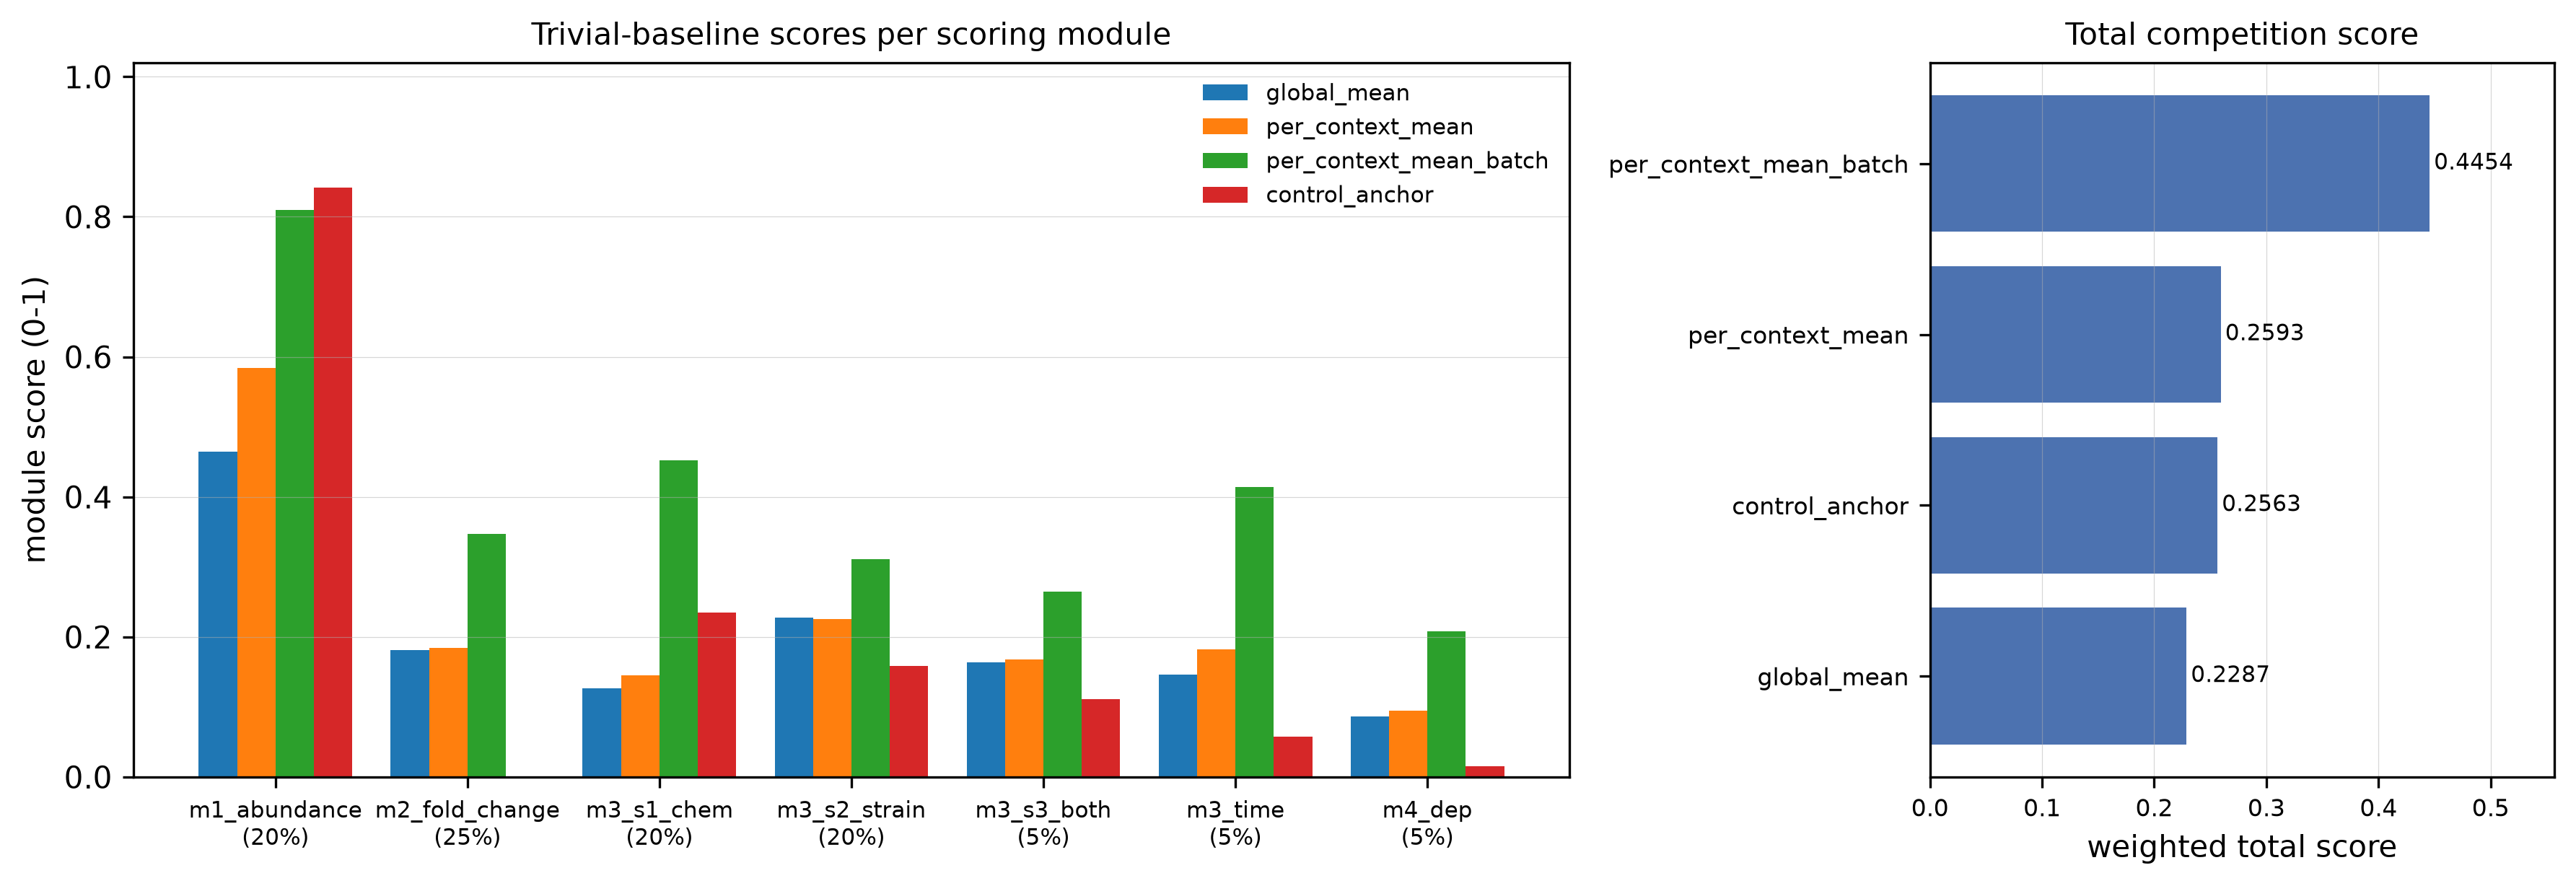
\includegraphics[width=0.88\textwidth]{figures/harness_baseline_scores.png}
\caption{\textbf{平凡基线的分模块与总分（验证队列）。} 左：四个基线在七个评分模块上的得分；右：加权总分。\code{per\_context\_mean\_batch}（按官方分组实现的均值基线，总分 0.445443）在 M1 上高达 0.8094；而 \code{control\_anchor}（把 $\bm{\Delta}$ 预测为零）在 M2 上得 0，在残差模块上却仍有 0.06--0.24——这就是表 \ref{tab:rubric} 的空值下限。四个基线的总分分别为 0.228690（\code{global\_mean}）、0.259257（\code{per\_context\_mean}）、0.445443（\code{per\_context\_mean\_batch}）与 0.256303（\code{control\_anchor}）。}
\label{fig:baselines}
\end{figure}

\subsection{探索环境的引擎：快速代理评分器与等价性门}
\label{sec:fastscore}

权重搜索是全流程的计算瓶颈：精确评分一次需 20.01--27.29\,s，而坐标上升在 868 维权重空间上需十万量级评估。我们利用一个代数事实：候选预测对权重是仿射的，$\mathbf{P}=\mathbf{B}+\sum_k w_k\mathbf{F}_k$；由于成员矩阵处处有限、只有真值携带 NaN，\textbf{有限单元掩码不依赖权重}，因而评分所需的七个掩码共矩都是 $\bm{w}$ 的多项式，可一次预计算、常数时间重估。实测单次评估 0.004413\,s，\textbf{约 6\,184 倍加速}。

关键在于这个加速\textbf{不能靠信任}。代理与精确评分的一致性在优化器允许启动\emph{之前}被强制校验，容差 $10^{-6}$，用五个对抗性设计的权重张量（全零、簇常数、单簇置零、完全随机、0 与 1.2 交替）；实测最大偏差在 $1.2\times10^{-10}$--$3.4\times10^{-9}$ 之间。之所以需要「簇常数」以外的用例，是因为散射累加类的错误在簇常数张量下会自行抵消。Module 4（$|\Delta|>1$ 阈值）对权重不是多项式，因此被排除在快速路径外——\textbf{任何被报告为\emph{成绩}的分数都不来自快速路径}。

\subsection{研究信号一：S1 模块奖励的是批次复现（两个队列同向复现）}
\label{sec:s1confound}

\begin{keybox}[title=一个由探索环境自己发现的口径隐患]
\small
按官方分组实现的均值基线在验证队列 S1 上的残差相关为 \textbf{0.4528}。我们把式 \eqref{eq:resid} 中批次盲的 $\bm{\mu}_{\text{ctx}}$ 换成\textbf{批次感知}的版本后重新评分，该基线的 S1 \textbf{塌缩至 0.0004}，而梯度提升模型仍保留 0.1716。
\NEW{}\textbf{同一诊断在测试队列上复现}：同一基线的 S1 残差相关由 0.381 塌缩至 \textbf{0.014}（降幅 0.367），而我们提交的模型由 0.401 降至 0.192——降幅仅 0.208，且仍显著高于零。
换言之，「新化合物泛化」这一模块的\emph{基线优势}几乎全部来自复现批次条件均值，而非任何化学外推能力；我们的模型则有一个不能被批次解释的剩余部分。
这一发现改变了此后所有优化方向，也说明：\textbf{任何采用「减去群体均值再算残差相关」口径的扰动预测基准都可能存在同类隐患}。
\end{keybox}

这条信号的证据链是本方案最看重的一条，因为它\textbf{同时具备三个属性}：由自动断言而非人工阅读发现；在两个独立队列上同向复现（验证队列 $n=1\,065$、测试队列 $n=1\,640$）；并且指向一个可以被别人在自己的基准上重复检验的一般性问题。定量结果见图 \ref{fig:selfscore}F。

\subsection{研究信号二：\code{test\_time} 是时间插值而非外推}
\label{sec:timeinterp}

阶段 2 的一条断言失败暴露出一个口径事实：\code{val\_time} 划分\textbf{不是时间外推}——六个时间值在训练集中全部出现，该轴实为\emph{条件-时间网格补全}（插值），其中 62.59\,\% 的行含有新的（条件 $\times$ 时间）单元，其余 37.41\,\% 为同一单元的重复测量。我们在阶段 2 就据此把该模块重新标注为「时间插值」。

修订后的手册（2.2 节第 13 条）把场景表补列 \code{test\_time} 并明确其为\textbf{时间插值}、非外推，评分模块名称相应改为「双重未知 / 时间插值」——这与我们的独立发现一致。我们把这件事写进正文，不是为了自证，而是因为它说明一件方法学上的小事：\emph{划分的语义必须由断言检查，而不能由名称推断}。

\subsection{\NEW{}依据修订释放的测试集真值：七模块自评}
\label{sec:selfscore}

修订后手册第 2.2 节第 7 条明确：\textbf{测试集蛋白质组真值随数据包一并发布，供参赛队自评参考，不作最终排名依据}；最终评审另用一组不随赛题发放的独立内部评测集，晋级队伍须通过代码复现核验。这解除了我们在上一版文档中的一个限制——当时我们只能报告一个「指示性」的逐样本倍数变化相关（0.3844），无法给出总分。

本次我们用\textbf{完全相同}的离线口径在测试队列上计算了七模块总分。协议上有四条自我约束，写在脚本里而不是写在段落里：

\begin{enumerate}
\item \textbf{被评分的预测矩阵冻结于 2026-08-07}，早于本自评脚本存在；测试真值\textbf{只用于评分}，从未用于任何模型、权重、簇划分或超参数的选择。
\item $\bm{\mu}_{\text{ctx}}$、$\bm{\mu}_{\text{drug}}$ 与四个基线的分组均值\textbf{一律只在 \code{split\_final == 'train'} 行上拟合}。脚本内置一道硬性泄漏保护：把所有非训练行置空后重算，要求结果\textbf{逐位相同}，否则中止。该保护在本次运行中通过。
\item 报告口径与验证队列完全一致（规格版本 1.0.0），并同时给出四种聚合口径下的结果。
\item \textbf{这不是官方分数}：组委会的聚合口径与测试侧对照匹配规则未公开，且最终排名基于独立内部评测集。我们把这句话放在图题与表题里，而不是放在脚注里。
\end{enumerate}

\begin{figure}[H]
\centering
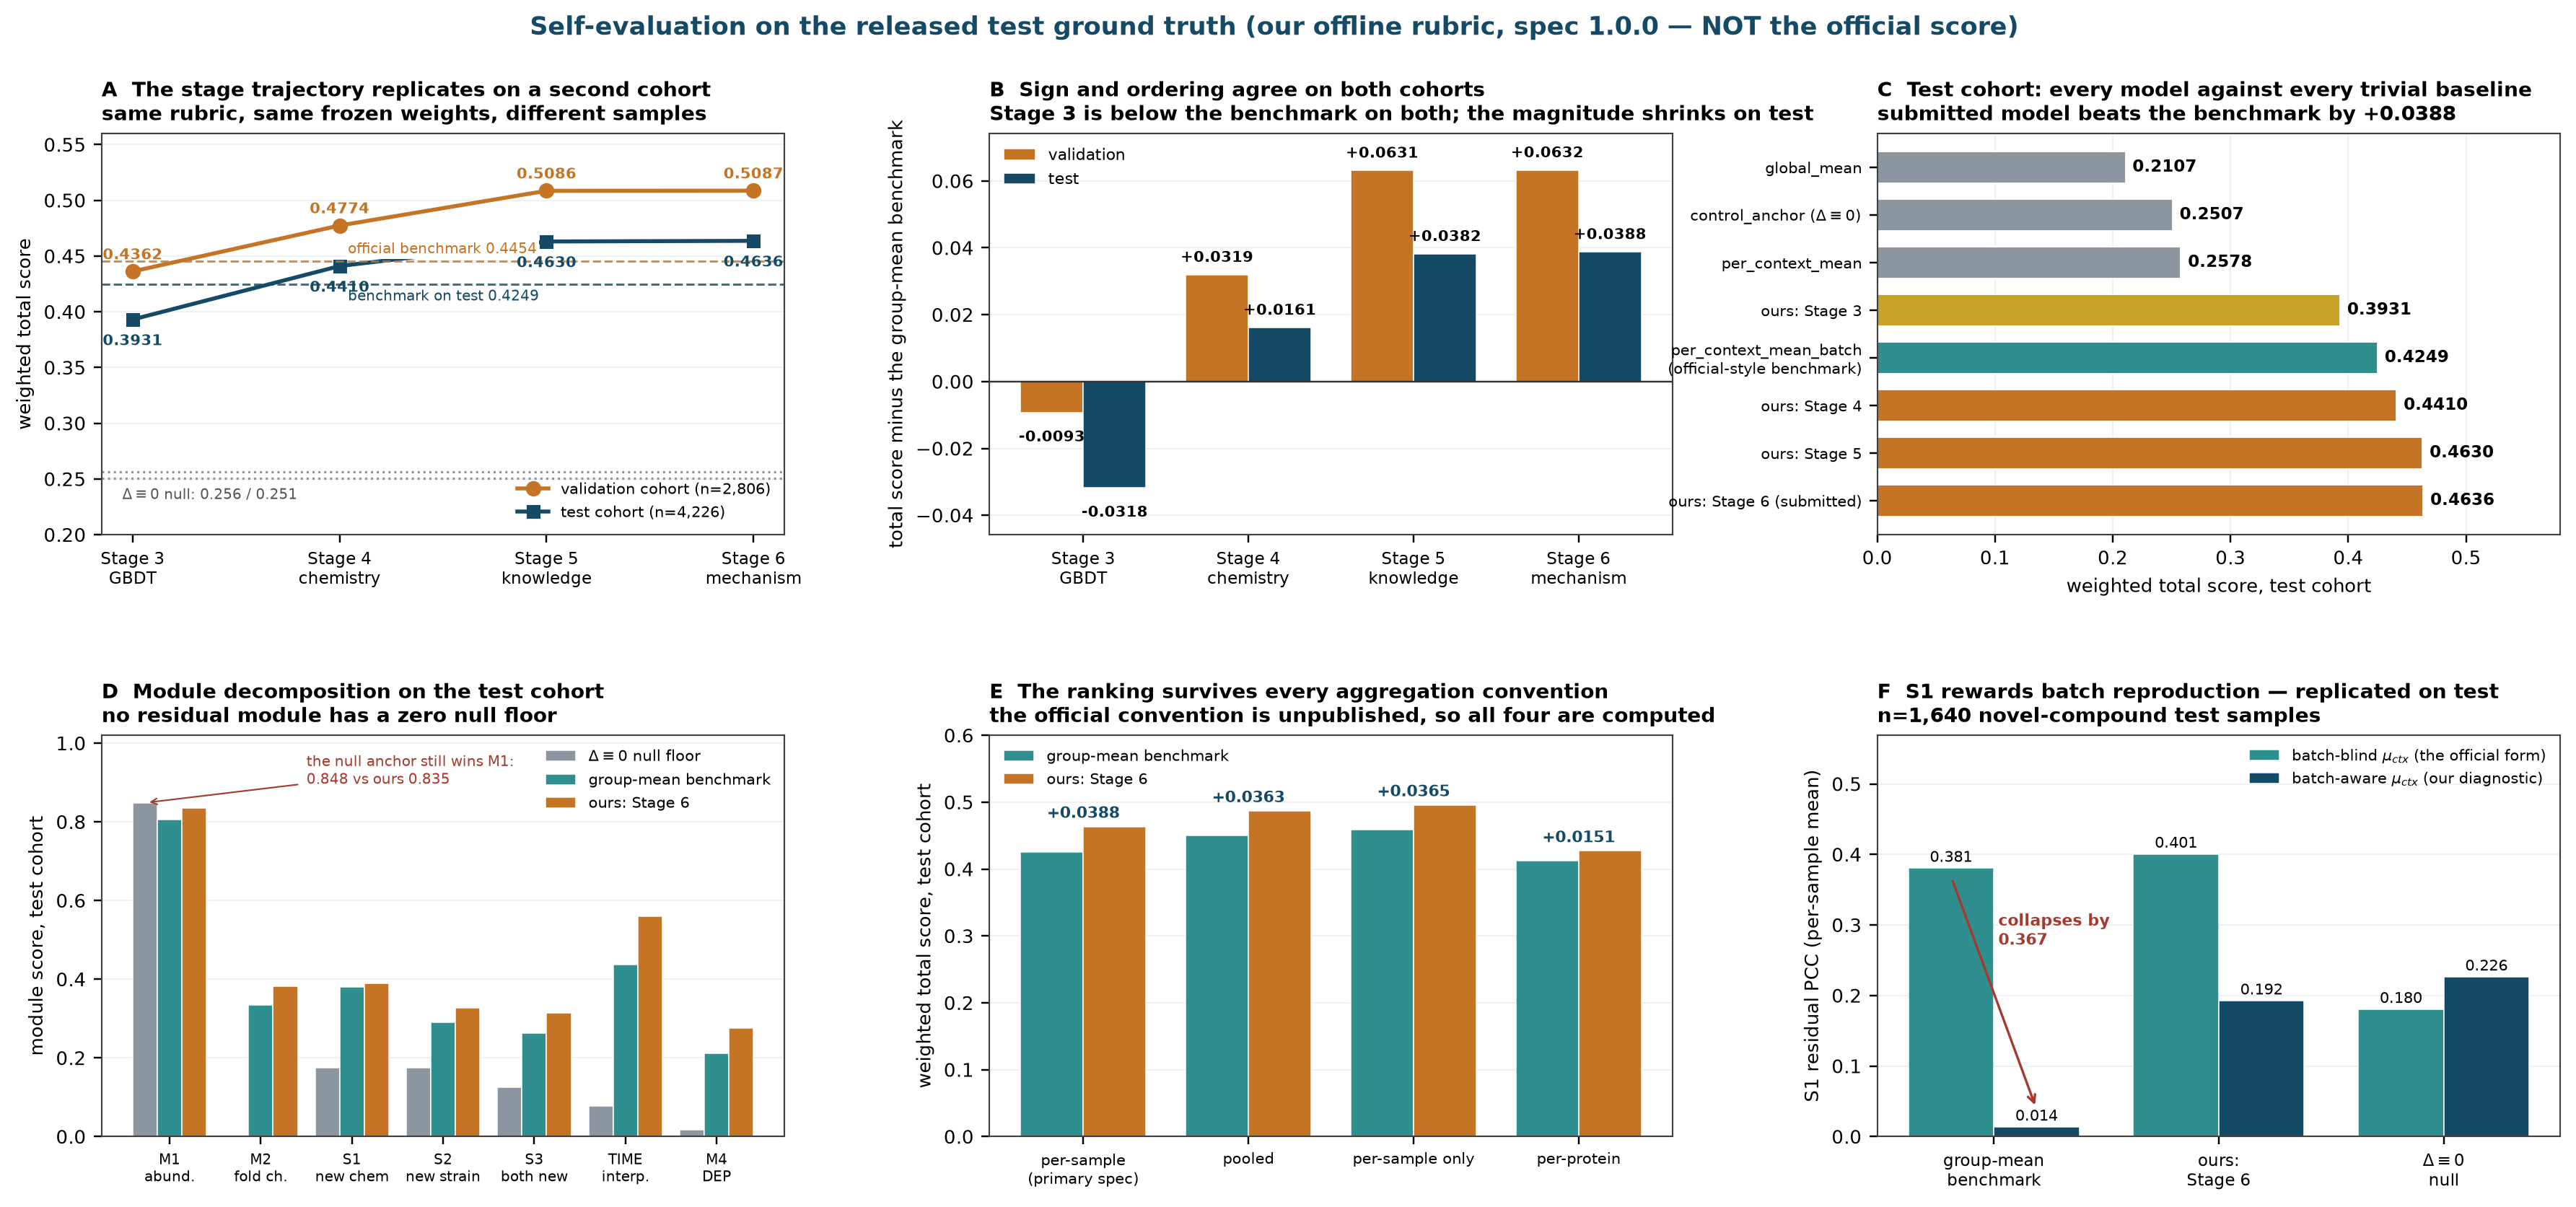
\includegraphics[width=\textwidth]{figures/step7_test_selfscore.png}
\caption{\textbf{测试队列七模块自评（全部数值由公开快照 \file{evidence/step7\_test\_selfscore.json} 在绘图时读入；这不是官方分数）。}
\textbf{A} 四个阶段在两个队列上的总分轨迹：\emph{同一套冻结权重、同一套口径、不同样本}，轨迹形状一致；
\textbf{B} 各阶段相对同口径分组均值基线的差值——阶段 3 在两个队列上\textbf{均低于}基线，阶段 4/5/6 在两个队列上\textbf{均高于}基线，且测试侧幅度系统性小于验证侧；
\textbf{C} 测试队列上八个预测器的总分；
\textbf{D} 测试队列的七模块分解，红色标注指出\emph{零假设锚点在 M1 上仍然胜过我们的模型}（0.8484 对 0.8348）；
\textbf{E} 四种聚合口径下我方相对基线的差值均为正（$+0.0151$ 至 $+0.0388$），说明排名对未公布的聚合口径稳健；
\textbf{F} S1 批次混杂诊断在测试队列上的复现（\S\ref{sec:s1confound}）。}
\label{fig:selfscore}
\end{figure}

\begin{table}[H]
\centering\small
\caption{\textbf{\NEW{}测试队列自评总表（离线口径，非官方分数）。} 八个预测器 $\times$ 七模块 $+$ 加权总分。\code{per\_context\_mean\_batch} 为按官方分组字段构造的均值基线。最后一列为相对该基线的总分差值。}
\label{tab:testscore}
\begin{adjustbox}{max width=\textwidth}
\begin{tabular}{lccccccc|cc}
\toprule
预测器 & M1 & M2 & S1 & S2 & S3 & TIME & M4 & 总分 & 相对基线 \\
\midrule
\code{global\_mean} & 0.4632 & 0.1638 & 0.0743 & 0.2130 & 0.1643 & 0.1429 & 0.0856 & 0.2107 & $-0.2142$ \\
\code{control\_anchor} & \textbf{0.8484} & 0.0000 & 0.1753 & 0.1752 & 0.1260 & 0.0768 & 0.0163 & 0.2507 & $-0.1742$ \\
\code{per\_context\_mean} & 0.6118 & 0.1833 & 0.1122 & 0.2195 & 0.1783 & 0.1851 & 0.1028 & 0.2578 & $-0.1670$ \\
阶段 3（GBDT） & 0.7254 & 0.3391 & 0.2935 & 0.2935 & 0.2495 & 0.4957 & 0.1717 & 0.3931 & $-0.0318$ \\
\code{per\_context\_mean\_batch} & 0.8065 & 0.3351 & 0.3806 & 0.2905 & 0.2623 & 0.4378 & 0.2120 & 0.4249 & 基准 \\
阶段 4（分子化学） & 0.8249 & 0.3567 & 0.3564 & 0.3019 & 0.2706 & 0.5662 & 0.2673 & 0.4410 & $+0.0161$ \\
阶段 5（知识图谱） & 0.8346 & 0.3816 & 0.3900 & 0.3266 & 0.3126 & 0.5584 & 0.2771 & 0.4630 & $+0.0382$ \\
\textbf{阶段 6（提交）} & 0.8348 & 0.3824 & \textbf{0.3900} & \textbf{0.3278} & \textbf{0.3143} & \textbf{0.5599} & 0.2759 & \textbf{0.4636} & $\bm{+0.0388}$ \\
\bottomrule
\end{tabular}
\end{adjustbox}
\end{table}

\begin{okbox}[title=测试队列自评给出的三条读数]
\small
\begin{enumerate}
\item \textbf{结论方向在第二个队列上成立}。阶段轨迹的\emph{符号与次序}在两个队列上一致：阶段 3 均低于基线（验证 $-0.0093$、测试 $-0.0318$），阶段 4/5/6 均高于基线（验证 $+0.0319/+0.0631/+0.0632$，测试 $+0.0161/+0.0382/+0.0388$）。这是一次跨队列的独立复算，而非同一队列的重复报告。
\item \textbf{幅度在测试队列上系统性缩小}（$+0.0632\to+0.0388$）。我们不把这解释为「过拟合」——所有权重都在折外队列上拟合、验证集只评分一次——而更可能是队列构成差异：测试队列含\emph{两个}未见菌株的双新划分（1\,129 例）与 11 个新化合物，外推压力高于验证队列。这一解释可被检验，但\textbf{尚未检验}。
\item \textbf{零假设锚点在 M1 上仍胜过我们}（0.8484 对 0.8348）。这是一个我们没有解决的问题，写在这里而不是隐藏在附录：一个更好的方案应当在\emph{不牺牲} M2/S1/S2 的前提下夺回 M1，例如按逐单元不确定度向对照锚点收缩（\S\ref{sec:tobit} 与表 \ref{tab:plan} 工作项 C）。
\end{enumerate}
\end{okbox}
